\renewcommand{\thesection}{\Alph{section}}
\setcounter{figure}{0}
\renewcommand{\thefigure}{\Alph{section}.\arabic{figure}}
\appendix
\addchap{Anhang}

\captionsetup{list=false}

\section{Bilder}
\begin{figure}[H]
\centering
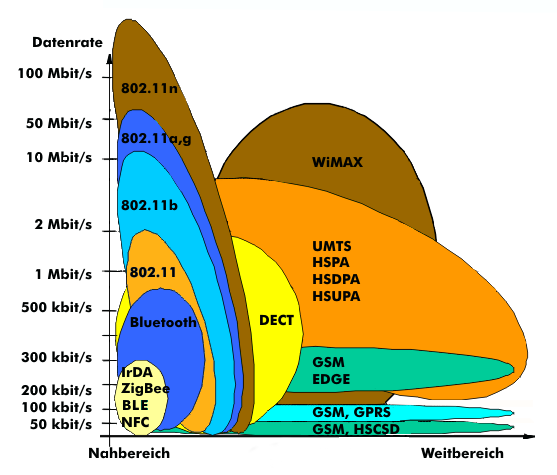
\includegraphics[scale=1]{Bilder/Funktechnologien.png} 
\caption{Überblick zu heutigen Funktechnologien \cite{FUE}}
\label{fig:FUE}
\end{figure}
\begin{figure}[H] 
\centering
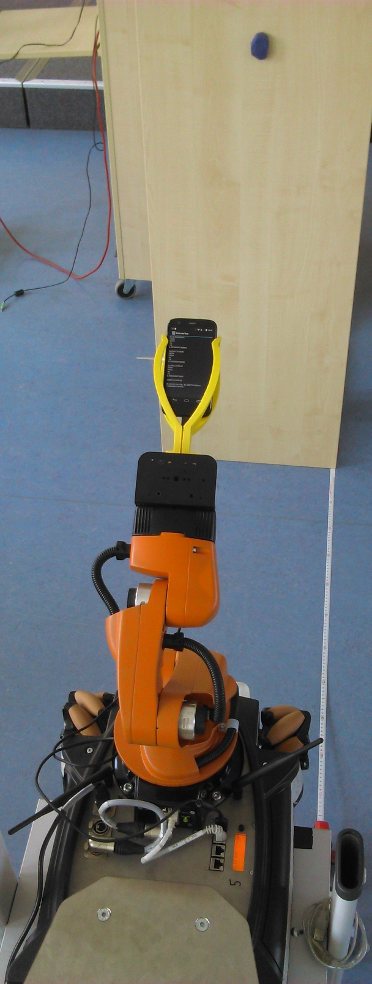
\includegraphics[scale=0.3]{Bilder/MessungDistanz1}
\caption{Distanz-Signalstärke-Messung Bild 1}
\label{fig:MessungDistanz1}
\end{figure}
\begin{figure}[H] 
\centering
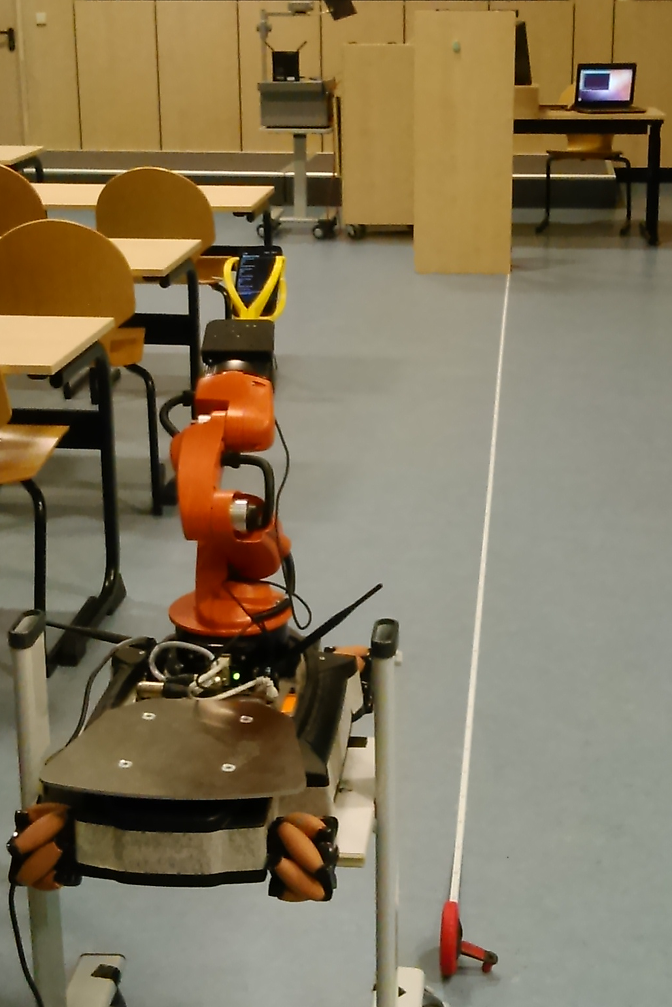
\includegraphics[scale=0.3]{Bilder/MessungDistanz2}
\caption{Distanz-Signalstärke-Messung Bild 2}
\label{fig:MessungDistanz2}
\end{figure}
\begin{figure}[H] 
\centering
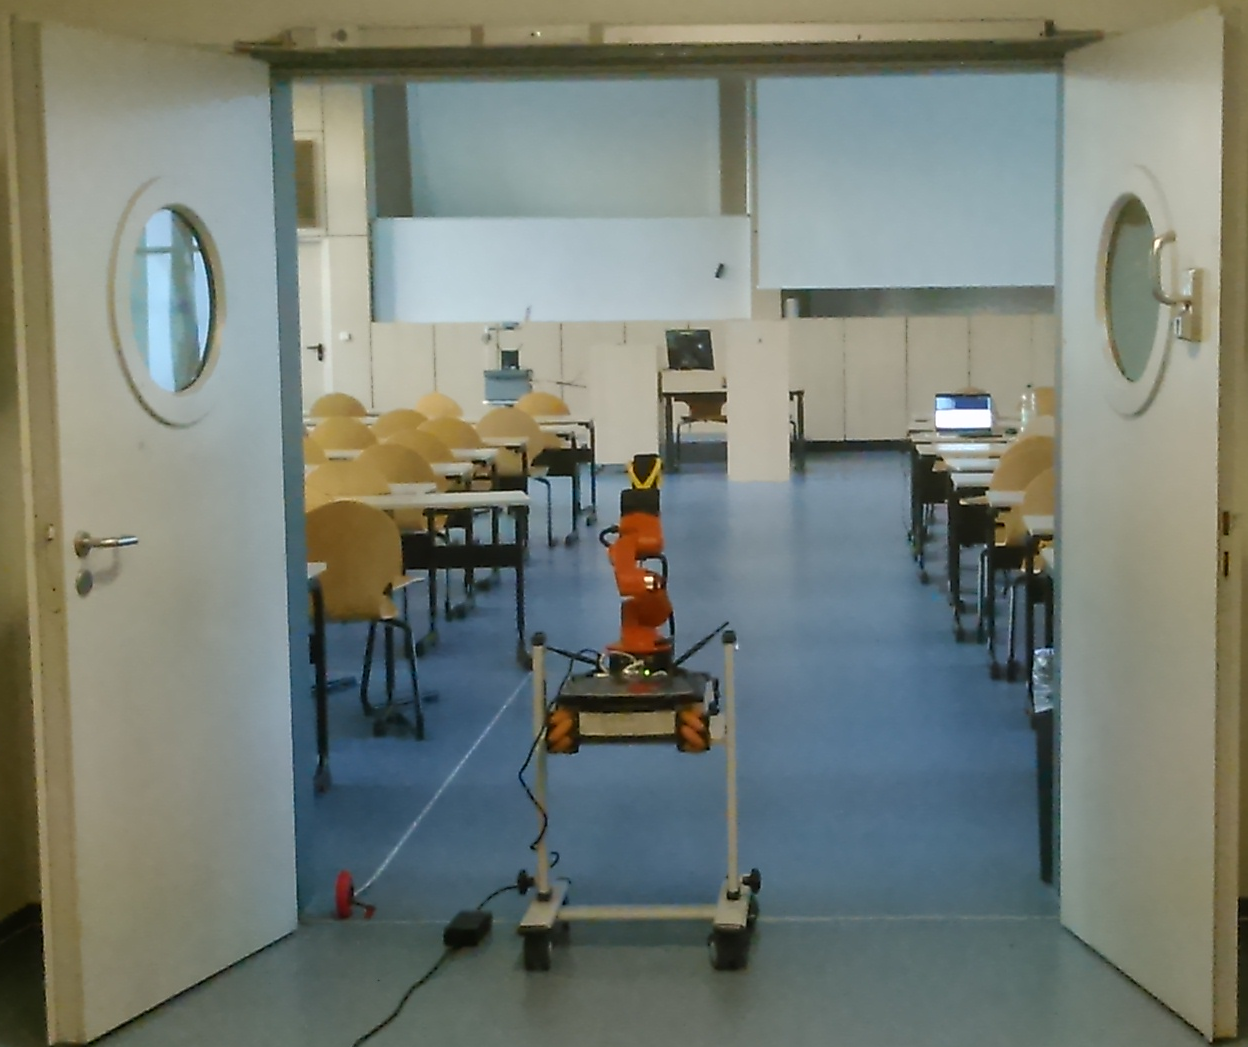
\includegraphics[scale=0.3]{Bilder/MessungDistanz3}
\caption{Distanz-Signalstärke-Messung Bild 3}
\label{fig:MessungDistanz3}
\end{figure}

%\begin{figure}[H] 
%\centering
%\begin{tikzpicture}
%\begin{groupplot}[group style={group name=my plots, group size=1 by 4,ylabels at=edge left, vertical sep= 1.5cm}, width=0.7\paperwidth, height=0.15\paperheight, tickpos=left, ytick align=outside, xtick align=outside, enlarge x limits=false]
%\nextgroupplot[title={Beacon in 1 Meter Entfernung},xticklabels={,,}]
%\addplot[color=dblue] table [col sep=comma] {TikzDaten/DrehungEinzeln1.dat};
%\nextgroupplot[title={Beacon in 5 Metern Entfernung},ylabel={Empfangene Signalstärke in dBm},xticklabels={,,}]
%\addplot[color=ice] table [col sep=comma] {TikzDaten/DrehungEinzeln5.dat};
%\nextgroupplot[title={Beacon in 10 Metern Entfernung},xticklabels={,,}]
%\addplot[color=mint] table [col sep=comma] {TikzDaten/DrehungEinzeln10.dat};
%\nextgroupplot[title={Orientierung in Z-Richtung},xlabel={Zeit in Sekunden},ylabel={Lage in Grad}]
%\addplot[solid] table [col sep=comma] {TikzDaten/DrehungAusrichtung.dat};
%\end{groupplot}
%\end{tikzpicture}
%\caption{Verlauf der gemessenen Signalstärke eines Beacons in verschiedenen Distanzen zu der Drehung des Smartphones in Z-Richtung über die Zeit}
%\label{fig:DrehungEinzeln}
%\end{figure}

(1 Bild noch mit den drei ausgewählten Distanzen 1, 5 und 10 Meter und dazu auch die Drehwinkel) - Hier ebenso wie oben alles schön erklären und auch auf die Streuung eingehen, also ob die Signaleintrübung immer gleich blieb oder auch über die Distanz zunahm.
\section{Tabellen}


\section{App-Aufbau}
Anhang für die einzelnen App-Bestandteile.

